\section{Introduction}
Canonical correlation analysis (CCA) is a joint multidimensional dimensionality reduction
algorithm for two exactly two datasets \cite{hotelling1936relations}. CCA finds a linear
transformation for each dataset such that the correlation between the two transformed
features is maximized. The basis vectors that span the subspaces of these transformations
are called canonical vectors. While CCA itself is not a data fusion algorithm, the
correlated features that it returns may be used in data fusion algorithms.  Such data
fusion algorithms are becoming a necessity with the increased ability to capture
high-dimensional multi-modal datasets, arising in fields such as computer vision
\cite{hardoon2004canonical, dhillon2011multi,
  lisanti2014matching,ahsan2014clustering,hardoon2006correlation,chaudhuri2009multi}, and
medical signal processing, \cite{khalid2013improving, correa2010canonical,
  seoane2014canonical, spuler2013spatial, chen2014removal}.

However, in many applications, the covariance matrices needed to solve CCA are
unknown and must be estimated from training data. When using sample covariance
estimates from fewer samples than the combined dimensions of the datasets, empirical CCA
falsely reports a perfect correlation between the datasets and random linear
transformations for each dataset \cite{pezeshki2004empirical}. In this low-sample,
high-dimensionality regime, empirical CCA fails to reliably identify correlations between
the datasets. However, using insights from random matrix theory, Nadakuditi
\cite{nadakuditi2011fundamental} proposed informative CCA (ICCA), which overcomes this
performance loss to reliably identify correlations in the sample deficient regime.

In this paper, we consider the accuracy of the canonical vectors returned by empirical CCA
and ICCA and propose an improved estimate that we name \iccaps. Throughout, we assume that
each dataset is modeled with a low-rank signal-plus-noise data model, which is ubiquitous
in signal processing applications. We begin by deriving the CCA population canonical
vectors if all parameters are known. From this analysis we see that the canonical vectors
are a linear combination of signal vectors that form the linear signal subspace of each
dataset. Empirical CCA, ICCA, and \iccap all use different weights of an estimated signal
subspace. Importantly, \iccap relies on insights from random matrix theory that quantify
the accuracy of the signal subspace estimate, resulting in the most accurate
estimate. While the ICCA canonical vectors are suboptimal, they greatly improve upon the
canonical vectors of empirical CCA, which are random in the low-sample low-SNR regime.

This paper is organized as follows. We provide the linear low-rank signal-plus-noise data
model in Section \ref{sec:chpt5:model}. We then derive the solution of CCA and empirical
CCA in Section \ref{sec:chpt5:cca}. In Section \ref{sec:chpt5:rmt}, we provide the
necessary insights from random matrix theory to derive ICCA and our new algorithm \iccap
in sections \ref{sec:chpt5:icca} and \ref{sec:chpt5:iccap}, respectively. We
validate our main results on synthetic data in Section \ref{sec:chpt5:emp} and provide
concluding remarks in Section \ref{sec:chpt5:conc}.

\section{Data Model}\label{sec:chpt5:model}

Throughout this paper, we consider the follow ubiquitous low-rank signal-plus-noise data
model. We assume that we are given $n$ observations of each dataset, which we stack columnwise to
form two data matrices
\beq\label{eq:chpt5:data}
 X = [x_1,\dots,x_n],\,\,\, Y = [y_1,\dots,y_n].
\eeq
For $i=1,\dots,n$, let $\xii\in\complex^{p\times 1}$
and $\yii\in\complex^{q\times 1}$ be modeled as
\beq\label{eq:chpt5:data_model}
\xii = \Ux\sx + \zx,\,\,\,\,\yii = \Uy\sy + \zy,
\eeq
where $\Ux^H\Ux=I_{\kx}$, $\Uy^H\Uy=I_{\ky}$, $\zx\simiid\mathcal{CN}(0,I_p)$ and
$\zy\simiid\mathcal{CN}(0,I_q)$. Furthermore, assume that
\be
\sx\sim\mathcal{CN}(0,\Tx),\,\,\,\,\sy\sim\mathcal{CN}(0,\Ty),
\ee
where
\begin{subequations}\label{eq:chpt5:thetas}
\beq
\Tx=\diag\left(\left(\tx_1\right)^2,\dots,\left(\tx_{\kx}\right)^2\right)
\eeq
\beq
\Ty=\diag\left(\left(\ty_{1}\right)^2,\dots,\left(\ty_{\ky}\right)^2\right).
\eeq
\end{subequations}
Assume that $\zx$ and $\zy$ are
mutually independent and independent from both $\sx$ and $\sy$. Finally, assume that
\be
\E{\sx \sy^H} \defeq \Kxy = \Tx^{1/2}\Pxy\Ty^{1/2},
\ee
where the entries of $\Pxy$ are $-1\leq |\rho_{kj}| \leq 1$ and represent the correlation
between $\sx^{(k)}$ and $\sy^{(j)}$. For reasons to be made clear later, define
\beq\label{eq:chpt5:kxytil}
\Kxytil = \left(\Tx+I_{\kx}\right)^{-1/2}\Kxy\left(\Ty+I_{\ky}\right)^{-1/2}.
\eeq
Under this model, we define the following
covariance matrices
\begin{subequations}\label{eq:chpt5:true_scm}
\beq\label{eq:chpt5:rxx}
\E{\xii\xii^H} = \Ux\Tx\Ux^H + I_p \defeq \Rxx
\eeq
\beq\label{eq:chpt5:ryy}
\E{\yii\yii^H} = \Uy\Ty\Uy^H + I_q \defeq \Ryy
\eeq
\beq\label{eq:chpt5:rxy}
\E{\xii\yii^H} = \Ux\Kxy\Uy^H \defeq \Rxy.
\eeq
\end{subequations}
Note that we may write $\sx=\Tx^{1/2} v_{x,i}$ and $\sy=\Ty^{1/2} v_{y,i}$ where
$v_{x,i}\sim\mathcal{CN}(0,I_{k_x})$ and $v_{y,i}\sim\mathcal{CN}(0,I_{k_y})$ are
independent random vectors. Defining $Z_n^x = [z_{x,1},\dots,z_{x,n}]$, $Z_n^y =
[z_{y,1},\dots,z_{y,n}]$, $\Vx=[v_{x,1},\dots,v_{x,n}]$, and $\Vy=[v_{y,1},\dots,v_{y,n}]$, we may write our data
matrices in (\ref{eq:chpt5:data}) as the sum of a low-rank signal matrix and noise
matrix
\beq\label{eq:chpt5:data_matrices}
 X = \Ux\Tx^{1/2}\Vx^H + Z_n^x,\,\,\,\, Y = \Uy\Ty^{1/2}\Vy^H + Z_n^y.
\eeq

Finally, denote the singular values of $Z_n^x$ and $Z_n^y$ as 
\be
\sigma_1(Z_n^x)\geq\cdots\geq\sigma_p(Z_n^x),\,\,\,\,
\sigma_1(Z_n^y)\geq\cdots\geq\sigma_q(Z_n^y)
\ee
where without loss of generality we let $p<n$ and $q<n$ to simplify the definition of the
empirical singular value distribution. Let $\mu_{Z_n^x}$ and $\mu_{Z_n^y}$ be the
empirical singular value distribution defined as
\be
\mu_{Z_n^x} = \frac{1}{p}\sum_{i=1}^p\delta_{\sigma_i(Z_n^x)},\,\,\,\, \mu_{Z_n^y} =
\frac{1}{q}\sum_{i=1}^q\delta_{\sigma_i(Z_n^y)}. 
\ee
Assume that the probability measures $\mu_{Z_n^x}$ and $\mu_{Z_n^y}$ converge almost
surely as $p,q,n\to\infty$ with $p/n\to c_x$ and $q/n\to c_y$ to non-random compactly
supported probability measures 
$\mu_{Z_x}$ and $\mu_{Z_y}$ respectively. Finally, we assume that $\sigma_1(Z_n^x)\convas
b_x$ and $\sigma_1(Z_n^y)\convas\ b_y$. 

\section{Canonical Correlation Analysis}\label{sec:chpt5:cca}

Canonical Correlation Analysis (CCA) is a dimensionality reduction algorithm that finds
linear projections for $\xii$ and $\yii$ such that in the projected spaces, the variables
are maximally correlated. Specifically, CCA solves the following optimization problem
\beq\label{eq:chpt5:opt_cca}
\rhocca =\max_{\wx,\wy} \frac{\wx^H\Rxy\wy}{\sqrt{\wx^H\Rxx\wx}\sqrt{\wy^H\Ryy\wy}},
\eeq
where $\wx$ and $\wy$ are called canonical vectors and $\rhocca$ is called the canonical
correlation coefficient. Notice that we can scale $\wx$ and
$\wy$ and still achieve the same objective function. Therefore, we may constrain the
canonical variates to have unit norm, resulting in 
\beq\label{eq:chpt5:cca}\ba
&\max_{\wx,\wy} &&\wx^H\Rxy\wy\\
&\text{subject to} && \wx^H\Rxx\wx = 1, \wy^H\Ryy\wy=1.\\
\ea\eeq
Substituting the change of variables $\wxt=\Rxx^{1/2}\wx$ and
$\wyt=\Ryy^{1/2}\wy$ in (\ref{eq:chpt5:cca}) results in the following optimization problem
\beq\label{eq:chpt5:cca_svd}\ba
&\max_{\wxt,\wyt} &&\wxt^H\Rxx^{-1/2}\Rxy\Ryy^{-1/2}\wyt\\
&\text{subject to} && \wxt^H\wxt = 1, \wyt^H\wyt=1.\\
\ea\eeq
Examining the optimization problem in (\ref{eq:chpt5:cca_svd}), we can immediately see that the
solution to CCA may be solved via the SVD of the matrix
\beq\label{eq:chpt5:c_cca}
\Ccca = \Rxx^{-1/2}\Rxy\Ryy^{-1/2}
\eeq
Define $\Ccca=FKG^T$ as the SVD of $\Ccca$ where $F$ is an unitary
$p\times p$ matrix with columns $f_1,\dots,f_p$, $G$ is a unitary $q\times q$ matrix with
columns $g_1,\dots,g_q$, and
$K=\diag(k_1,\dots,k_{\min(p,q)})$ is a $p\times q$ matrix whose diagonal elements are the
singular values of $\Ccca$. The solution to (\ref{eq:chpt5:cca_svd}) is
\be
\wxt = f_1,\,\,\,\,\wyt = g_1,\,\,\,\,\rho = k_1.
\ee
and the canonical vectors are
\beq\label{eq:chpt5:cca_vectors}
\wx = \Rxx^{-1/2}\wxt,\,\,\,\,\wy = \Ryy^{-1/2}\wyt.
\eeq
We can obtain higher order canonical correlations and vectors by taking successive singular
value and vector pairs.

\subsection{Population canonical vectors}

We first determine the population canonical vectors of our data model in
(\ref{eq:chpt5:data_model}). To do so, we need the singular vectors of 
\be\ba
& \Ccca  && = \Rxx^{-1/2}\Rxy\Ryy^{-1/2}\\
%&&& = \left(\Ux\Tx\Ux^H + I_{\kx}\right)^{-1/2}\Ux\Kxy\Uy^H\left(\Ux\Ty\Uy^H +
%  I_{\ky}\right)^{-1/2}\\
&&& = \Ux\left(\Tx + I_{\kx}\right)^{-1/2}\Kxy\left(\Ty + I_{\ky}\right)^{-1/2}\Uy^H\\
&&& = \Ux\Kxytil\Uy^H.\\
\ea\ee
Define $U_{\widetilde{K}}K_{\widetilde{K}}V_{\widetilde{K}}^H$ as the SVD of
$\Kxytil$. First observe that the rank of $\Ccca$ is
$k\defeq\min(\kx,\ky)$. Defining the matrices of the canonical vectors
$W_x=[\wx^{(1)},\dots,\wx^{(k)}]$ and  $W_y=[\wy^{(1)},\dots,\wy^{(k)}]$, we have that  
\begin{subequations}\label{eq:chpt5:pop_cca_vects}
\beq
W_x = \Ux\left(\Tx + I_{\kx}\right)^{-1/2}\Uktil
\eeq
\beq
 W_y = \Uy\left(\Ty + I_{\ky}\right)^{-1/2}\Vktil.
\eeq
\end{subequations}
Therefore, we see that the individual canonical vectors $\wx^{(i)}$ and $\wy^{(i)}$ are
linear combinations of the signal subspaces $\Ux$ and $\Uy$, respectively. The weights of
these linear combinations are dependent on $\Tx$, $\Ty$, $\Uktil$, and $\Vktil$. 

\subsection{Empirical CCA canonical vector estimates}

In many applications, we do not know the covariance matrices $\Rxx$, $\Ryy$, and $\Rxy$
\textit{a priori}. Therefore, we cannot find the population canonical vectors in
by forming $\Ccca$, but instead must estimate this matrix from training data. Given
the data matrices in (\ref{eq:chpt5:data}), we form the sample covariance matrices
$\Rxxhat = \frac{1}{n}XX^H$, $\Ryyhat = \frac{1}{n}YY^H$, and $\Rxyhat = \frac{1}{n}XY^H$.
Define the data SVDs of the matrices in (\ref{eq:chpt5:data}) as
\be
X = \Uxhat\Sigxhat\Vyhat^H,\,\,\,\, Y = \Uyhat\Sigyhat\Vyhat^H
\ee
and trimmed matrices
\begin{subequations}\label{eq:chpt5:cca_trimmed}
\be
 \Uxtil = \Uxhat\left(:,1:\min(p,n)\right),\,\,  \Vxtil =
 \Vxhat\left(:,1:\min(p,n)\right) 
\ee
\be
 \Uytil = \Uyhat\left(:,1:\min(q,n)\right),\,\, \Vytil =
 \Vyhat\left(:,1:\min(q,n)\right). 
\ee
\end{subequations}
Substituting the SVDs of sample analogs of the matrices in (\ref{eq:chpt5:c_cca}), reveals
the insight (\cite[Eq. (6)]{nadakuditi2011fundamental}) that the matrix $\Ccca$ can be
estimated as 
\beq\label{eq:chpt5:cccahat}
\Cccahat = \Uxtil\Vxtil^H\Vytil\Uytil^H.
\eeq

To estimate the population canonical vectors, we use the corresponding left and right singular vectors
of $\Cccahat$, denoted by $f_i$ and $g_i$ respectively, and substitute the sample covariance matrices into
(\ref{eq:chpt5:cca_vectors}) to achieve the estimates
\beq\label{eq:chpt5:cca_vects}
\widehat{w}_{x,i}^{\text{cca}} = \Rxxhat^{-1/2}f_i,\,\,\,\,
\widehat{w}_{y,i}^{\text{cca}} = \Ryyhat^{-1/2}g_i.
\eeq
Notice that the inner matrix product of $\Cccahat$ in (\ref{eq:chpt5:cccahat}) is
$\Vxtil^H\Vytil$. Define the SVD of this $\min(p,n)\times\min(q,n)$ matrix as
$\widetilde{U}_{\widetilde{K}}$$\widetilde{K}_{\widetilde{K}}$$\widetilde{V}_{\widetilde{K}}^H$. Using
this definition, the sample covariance matrices, and the identity
$f_i=\Uxtil\widetilde{U}_{\widetilde{K}}(:,i)$, we have that under the data model in
(\ref{eq:chpt5:data_model}) the empirical CCA population canonical vector estimate is
\be
\widehat{w}_{x,i}^{\text{cca}}  =\Uxtil\Sigxtil^{-1}\widetilde{U}_{\widetilde{K}}(:,i).
\ee
A similar expression may be found for $\widehat{w}_{y,i}^{\text{cca}}$. Stacking these
empirical CCA canonical vectors estimates in a matrix yields 
\beq\label{eq:chpt5:emp_cca_vects}
\widehat{W}_x^{\text{cca}} = \Uxtil\left(\Sigxtil\right)^{-1}\widetilde{U}_{\widetilde{K}},\,\,\,\,
\widehat{W}_y^{\text{cca}} = \Uytil\left(\Sigytil\right)^{-1}\widetilde{V}_{\widetilde{K}}.
\eeq
We note here that the singular values of the individual data matrices may be used to
estimate the SNRs via $\Txhat = \Sigxtil^2 - I$ and $\Tyhat=\Sigytil^2 - I$. 



\section{Pertinent Results from Random Matrix Theory}\label{sec:chpt5:rmt}

In empirical CCA, the canonical vector estimates in (\ref{eq:chpt5:emp_cca_vects}) use the
full data SVDs, which assumes that the rank of underlying signals are of rank $\min(p,n)$
and $\min(q,n)$, respectively. This is obviously quite incorrect given our data model in
(\ref{eq:chpt5:data_model}). Important advances in random matrix theory allow us to
quantify the accuracy of the singular values and singular vectors of the individual data
matrices, $X$ and $Y$, used in the empirical CCA canonical vector estimates. These
insights from random matrix theory motivate a new algorithm to estimate the canonical
vectors. In this section, we provide the pertinent results needed for our new estimation
algorithm. 

Let $X$ be a data matrix as in (\ref{eq:chpt5:data}) modeled as in
(\ref{eq:chpt5:data_model}). For this section, we drop the subscript dependent on $x$ to
ease notation and assume, without loss of generality, that
$\theta_1\geq\theta_2\geq\cdots\geq\theta_{k}$. Let
$\widehat{U}\widehat{\Sigma}\widehat{V}^H$ be the SVD of $X$. We define the
D-transform of a probability measure $\mu$, depending on $c$, for $z>b$ as
\beq\label{eq:chpt5:d_trans}
\ba
&D_{\mu}(z) \defeq
&&\left[\int\frac{z}{z^2-t^2}d_{\mu}(t)\right]\times\\&&&\left[c_x\int\frac{z}{z^2-t^2}d_{\mu(t)}
+ \frac{1-c_x}{z}\right]\\
\ea\eeq
In the proposition below, $D^{-1}_{\mu}(\cdot)$ will denote its function inverse on $[b,+\infty)$.

%\begin{prop}\label{prop:rmt_sigma}
%Let $p,n\to\infty$ such that $p/n\to c$. Then for each $1\leq i\leq k$
%\beq\label{eq:chpt5:rmt_sig}
%\widehat{\sigma}_i\convas\begin{cases}D_{\mu_Z}^{-1}\left(\frac{1}{\theta_i^2}\right) &
%  \text{if } \theta_i^2>1/D_{\mu_Z}\left(b^+\right) \\ b& \text{otherwise}.\end{cases}
%\eeq
%\end{prop}

\begin{prop}\label{prop:rmt_uv}
Let $p,n\to\infty$ such that $p/n\to c$. Let $\widehat{u}_i$ and $\widehat{v}_i$ be the
left and right singular vectors, respectively, 
associated with the singular value $\widehat{\sigma}_i$. Then for ach $1\leq i\leq k$
\beq\label{eq:chpt5:rmt_u}
\alpha_i\defeq|\langle
\widehat{u}_i,u_i\rangle|^2\convas \begin{cases}
  \frac{-2\varphi_{\mu_Z}\left(\rho\right)}{\theta_i^2D^\prime_{\mu_Z}\left(\rho\right)}  
  &\theta_i^2>1/D_{\mu_Z}\left(b^+\right)\\ 0 & \text{otherwise}\end{cases} 
\eeq
\beq\label{eq:chpt5:rmt_v}
\beta_i\defeq|\langle
\widehat{v}_i,v_i\rangle|^2\convas \begin{cases}
  \frac{-2\varphi_{\widetilde{\mu}_Z}\left(\rho\right)}{\theta_i^2D^\prime_{\mu_Z}\left(\rho\right)} 
& \theta_i^2>1/D_{\mu_Z}\left(b^+\right)\\ 0 & \text{otherwise}\end{cases} 
\eeq
where $\rho = D_{\mu_Z}^{-1}\left(1/\theta_i^2\right)$,
$\widetilde{\mu}_Z=c\mu_Z+(1-c)\delta_0$, and for any probability measure $\mu$,
\beq\label{eq:chpt5:varphi_mu}
\varphi_\mu\left(z\right) \defeq \int\frac{z}{z^2-t^2}d\mu\left(t\right).
\eeq
\end{prop}

Proposition \ref{prop:rmt_uv} gives asymptotic results for the accuracy of the singular
vectors of a data matrix. These results rely on the D-transform of the noise matrix
$Z$. This transform is invariant to orthogonal transformations, and so only depends on the
singular values of $Z$ and so we may assume, without loss of generality, that $Z$ is
diagonal.  Given the data matrix $X$, its SVD $\widehat{U}\widehat{\Sigma}\widehat{V}^H$,
and an estimate of the rank of $X$, $\widehat{k}$, we first form an estimate of $Z$ by
forming the truncated matrix \beq\label{eq:chpt5:Zhat} \widehat{Z} =
\diag\left(\widehat{\sigma}_{\widehat{k}+1},\dots,\widehat{\sigma}_p\right).  \eeq Using
this estimate, we may estimate the asymptotic D-transform at a point $z$ and its
derivative by following \cite{nadakuditi2014optshrink} via (\ref{eq:chpt5:Dhat}) and (\ref{eq:chpt5:Dprimehat}).
\begin{figure*}
\beq\label{eq:chpt5:Dhat}
\widehat{D}\left(z,\widehat{Z}\right)\defeq \frac{1}{p}\Tr\left(z\left(z^2I_p -
    \widehat{Z}\widehat{Z}^H\right)^{-1}\right)\cdot
\frac{1}{n}\Tr\left(z\left(z^2I_n-\widehat{Z}^H\widehat{Z}\right)^{-1}\right) \eeq
\beq\label{eq:chpt5:Dprimehat} \small
\begin{split}
\widehat{D}^\prime(z;\widehat{Z}) \defeq &\frac{1}{p}\Tr\left(z\left(z^2I_p -
    \widehat{Z}\widehat{Z}^H\right)^{-1}\right)\cdot
\frac{1}{m}\Tr\left(-2z^2\left(z^2I_m-\widehat{Z}^H\widehat{Z}\right)^{-2}+\left(z^2I_n -
    \widehat{Z}^H\widehat{Z}\right)^{-1}\right) + \\
&\frac{1}{m}\Tr\left(z\left(z^2I_m-\widehat{Z}^H\widehat{Z}\right)^{-1}\right)\cdot \frac{1}{n}\Tr\left(-2z^2\left(z^2I_p-\widehat{Z}\widehat{Z}^H\right)^{-2}+\left(z^2I_p-\widehat{Z}\widehat{Z}^H\right)^{-1}\right).
\end{split}
\eeq
\end{figure*}
We note that since $\widehat{Z}$ is a diagonal matrix, these expressions are extremely
efficient to compute. Similarly, we may estimate $\varphi_{\mu_Z}(z)$ and
$\varphi_{\widetilde{\mu}_Z}$ in (\ref{eq:chpt5:varphi_mu}) as
\beq\label{eq:chpt5:varphi_mu_hat}
\widehat{\varphi}_\mu\left(z;\widehat{Z}\right) =
\frac{1}{p}\Tr\left(z\left(z^2-\widehat{Z}\widehat{Z}^H\right)^{-1}\right) 
\eeq
and
\beq\label{eq:chpt5:varphi_mut_hat}
\widehat{\varphi}_{\widetilde{\mu}}\left(z;\widehat{Z}\right) =
\frac{1}{p}\Tr\left(z\left(z^2-\widehat{Z}^H\widehat{Z}\right)^{-1}\right). 
\eeq

With these data driven estimates, we can estimate $\theta_i$ and the
accuracies in Proposition \ref{prop:rmt_uv}.
%\beq\label{eq:chpt5:thetahat}
%\widehat{\theta}^2_i = \frac{1}{\frac{1}{p}\Tr\left(\widehat{\sigma}_i\left(\widehat{\sigma}_%i^2I_p -
%    \widehat{Z}\widehat{Z}^H\right)^{-1}\right)\cdot
%\frac{1}{n}\Tr\left(\widehat{\sigma}_i\left(\widehat{\sigma}_i^2I_n
%    -\widehat{Z}^H\widehat{Z}\right)^{-1}\right)}.
%\eeq
Using (\ref{eq:chpt5:Dhat}), (\ref{eq:chpt5:Dprimehat}),
(\ref{eq:chpt5:varphi_mu_hat}), (\ref{eq:chpt5:varphi_mut_hat}), the equality
$\frac{1}{\theta_i^2} = D_{\mu_Z}(\rho)$, and the consistent estimate
$\widehat{\sigma}_i\convas\rho$, we may estimate
\beq\label{eq:chpt5:alphahat}
\widehat{\alpha}_i = \frac{-2\widehat{\varphi}_\mu\left(\widehat{\sigma}_i,\widehat{Z}\right)\widehat{D}\left(\widehat{\sigma}_i,\widehat{Z}\right)}{\widehat{D}^\prime\left(\widehat{\sigma}_i,\widehat{Z}\right)}
\eeq
and
\beq\label{eq:chpt5:betahat}
\widehat{\beta}_i =
\frac{-2\widehat{\varphi}_{\widetilde{\mu}}\left(\widehat{\sigma}_i,\widehat{Z}\right)\widehat{D}\left(\widehat{\sigma}_i,\widehat{Z}\right)}{\widehat{D}^\prime\left(\widehat{\sigma}_i,\widehat{Z}\right)}. 
\eeq

\section{Informative CCA (ICCA)}\label{sec:chpt5:icca}

As an alternative to empirical CCA, we consider informative CCA (ICCA)
\cite{nadakuditi2011fundamental}, an algorithm that first trims the singular vectors of
the individual datasets to only include \textit{informative} singular vectors. Let
$\kxhat$ and $\kyhat$ be estimates of the number of informative components in $X$ and $Y$
respectively. Then define the trimmed data matrices
\begin{subequations}\label{eq:chpt5:trimmed_matrices}
\beq
 \Uxcir = \Uxhat\left(:,1:\kxhat\right),  \Uycir = \Uyhat\left(:,1:\kyhat\right)
\eeq
\beq
 \Vxcir = \Vxhat\left(:,1:\kxhat\right),
 \Vycir = \Vyhat\left(:,1:\kyhat\right)
\eeq
\beq
 \Sigxcir = \Sigxhat\left(1:\kxhat,1:\kxhat\right),
 \Sigycir = \Sigyhat\left(1:\kyhat,1:\kyhat\right).
\eeq
\end{subequations}
With these definitions, we define the ICCA matrix \beq\label{eq:chpt5:cicca}
\Ciccahat =
\Uxcir\Vxcir^H\Vycir\Uycir^H
\eeq
with SVD 
$\widehat{U}_{\widetilde{K}}\widehat{\Sigma}_{\widetilde{K}}\widehat{V}_{\widetilde{K}}$. 
Substituting these definitions in (\ref{eq:chpt5:pop_cca_vects}) yields the
ICCA population canonical vector estimates
\begin{subequations}\label{eq:chpt5:plugin_cca_vects}
\beq
\widehat{W}_x^{\text{icca}} = \Uxcir\left(\Txhat + I_{\kxhat}\right)^{-1/2}\Uktilhat
\eeq
\beq
\widehat{W}_y^{\text{icca}} = \Uycir\left(\Tyhat + I_{\kyhat}\right)^{-1/2}\Vktilhat.
\eeq
\end{subequations}

Similar to the population canonical vectors, the ICCA canonical
vector estimates correctly take only a linear combination of a few signal vectors. The
weighting is dependent on the estimates $\Txhat$, $\Tyhat$, $\widehat{U}_{\widetilde{K}}$,
and $\widetilde{V}_{\widetilde{K}}$. 

\section{\iccap}\label{sec:chpt5:iccap}
We expect the ICCA canonical vector estimates in (\ref{eq:chpt5:plugin_cca_vects}) to
greatly outperform the empirical CCA estimates in (\ref{eq:chpt5:emp_cca_vects}). However,
we still expect the estimates in (\ref{eq:chpt5:plugin_cca_vects}) to be suboptimal
because they substitute the signal subspace estimates, $\Uxhat$ and $\Uyhat$, without
considering their accuracy, which we quantified in Proposition \ref{prop:rmt_uv}. The
population, empirical CCA, and ICCA canonical vector estimates all take a linear
combination of the known or estimated signal subspace. With this observation, we consider
the following canonical vector estimates
\begin{subequations}\label{eq:chpt5:opt_cca_vects} 
\beq
\widehat{w}_{x,i}^{\text{icca+}} = \Uxcir\diag\left(\lambda_{x,i}^{\text{opt}}\right)\Uktilhat\left(:,i\right)
\eeq
\beq
\widehat{w}_{y,i}^{\text{icca+}} = \Uycir\diag\left(\lambda_{y,i}^{\text{opt}}\right)\Vktilhat\left(:,i\right),
\eeq
\end{subequations}
where 
$\lambda_{x,i}^{\text{opt}}=\left[\lambda_{x,i}^{(1)},\dots,\lambda_{x,i}^{(\kx)}\right]$ and
$\lambda_{y,i}^{\text{opt}}=\left[\lambda_{y,i}^{(1)},\dots,\lambda_{y,i}^{(\ky)}\right]$ and are the
solutions to the following optimization problems
\begin{subequations}\label{eq:chpt5:can_vec_opt_prob}
\beq
\lambda_{x,i}^{\text{opt}} = \argmin_{\lambda_x}\left\|w_x^{(i)} -
  \Uxhat\diag(\lambda_x)\Uktilhat\left(:,i\right)\right\|_F
\eeq
\beq
\lambda_{y,i}^{\text{opt}} = \argmin_{\lambda_y}\left\|w_y^{(i)} -
  \Uyhat\diag(\lambda_x)\Vktilhat\left(:,i\right)\right\|_F.
\eeq
\end{subequations}

This matrix approximation is similar to \cite{nadakuditi2014optshrink}, which examines the
optimal approximation to a signal matrix from noisy observations. Nadakuditi shows that
the classical Eckart-Young-Mirsky (EYM) low-rank matrix approximation is suboptimal when
trying to estimate a low-rank signal matrix from a low-rank signal-plus-noise matrix. The
EYM approximation is the optimal low-rank approximation of the low-rank signal-plus-noise
matrix but \textit{not} the low-rank signal matrix. Similarly here, the ICCA estimates
find the best representation of noisy canonical vectors and not the true underlying
canonical vectors. Instead we want the optimal estimates of the population canonical
vectors. The following proposition provides the closed form, deterministic answer to the
optimization problem for the \iccap weights.

\begin{prop}\label{prop:iccap}
The solutions to (\ref{eq:chpt5:can_vec_opt_prob}) are given by
\begin{subequations}\label{eq:chpt5:can_opt_sol}
\beq
\lambda_{x,i}^{\text{opt}} =
\diag\left(\Uxcir^H\Ux\left(\Tx+I_{\kx}\right)^{-1/2}\right)
\eeq
\beq
\lambda_{y,i}^{\text{opt}} =
\diag\left(\Uycir^H\Uy\left(\Ty+I_{\ky}\right)^{-1/2}\right).
\eeq
\end{subequations}
\end{prop}

The first key observation of this proposition is that the optimal weights are the same for
each subsequent canonical vectors (i.e. independent of $i$). The second key observation is
that the optimal weights are dependent on the matrix products $\Uxcir^H\Ux$ and
$\Uycir^H\Uy$. The diagonal elements of these matrices are the accuracies of the estimated
components of our signal subspaces that we asymptotically quantified in Proposition
\ref{prop:rmt_uv}. It makes sense then that the optimal weights tell us to place less
weight on inaccurately estimated signal subspaces. 

Next we provide the asymptotic limit of
the optimal weights in Proposition \ref{prop:iccap}. The analysis relies on the asymptotic
limit of the subspace accuracy provided in Proposition \ref{prop:rmt_uv}.

\begin{figure*}
\begin{Th}
  The solution to the optimal \iccaps weights in (\ref{eq:chpt5:can_opt_sol}) exhibits the following behavior
  in the asymptotic regime where $p,q,n\to\infty$ with $p/n\to c_x$ and $q/n\to c_y$.

  For $i=1,\dots,\kx$,
  \be
  \lambda_{x,\text{opt}}^{(i)} \convas 
  \begin{cases}
    D_{\mu_{Z_x}}\left(\sigma_x^{(i)}\right)\sqrt{\frac{-2\varphi_{\mu_{Z_x}}\left(\sigma_x^{(i)}\right)
      }{D^{\prime}_{\mu_{Z_x}}\left(\sigma_x^{(i)}\right)
        \left(1+D_{\mu_{Z_x}}\left(\sigma_x^{(i)}\right)\right)}} & \text{if }
    \left(\tx_i\right)^2 > 1/D_{\mu_{Z_x}}(b_x^+)\\ 
    0 & \text{otherwise} \\ \end{cases}
  \ee
  where $\sigma_x^{(i)}=D_{\mu_{Z_x}}^{-1}\left(1/\left(\tx_i\right)^2\right)$
and the  D-transform is defined in (\ref{eq:chpt5:d_trans}). A similar expression for
$\lambda_{y,\text{opt}}$ exists by replacing subscripts of $x$ with $y$. 
  \label{th:vect_opt}

\end{Th}
\end{figure*}

Theorem \ref{th:vect_opt} highlights some key differences between the ICCA and \iccaps. While
ICCA places positive weight on all subspace components, \iccaps will place place zero
weight on any subspace component that is \textit{uninformative}. We expect \iccap to
perform better than ICCA in this uninformative regime since it places no weight on
estimated subspaces that are simply noise. This theorem provides the asymptotic form of
the optimal weights to use in \iccap. To achieve a realizable estimate, we may use (\ref{eq:chpt5:Dhat}), (\ref{eq:chpt5:Dprimehat}),
(\ref{eq:chpt5:varphi_mu_hat}), and (\ref{eq:chpt5:varphi_mut_hat}) to estimate
\be
\widehat{\lambda}_{x,\text{opt}}^{(i)} =
  \widehat{D}\left(\widehat{\sigma}_x^{(i)},\widehat{Z}_x\right)\sqrt{\frac{-2\widehat{\varphi}\left(\widehat{\sigma}_x^{(i)},\widehat{Z}_x\right)
    }{\widehat{D}^{\prime}\left(\widehat{\sigma}_x^{(i)},\widehat{Z}_x\right)
      \left(1+\widehat{D}\left(\widehat{\sigma}_x^{(i)},\widehat{Z}_x\right)\right)}}
\ee

\section{Empirical Results}\label{sec:chpt5:emp}

In this section, we explore the accuracy of the ICCA and \iccap canonical vectors as
compared to those of CCA. We consider a rank-2 setting where $\kx=\ky=2$, $p=200$, $q=250$,
$\Tx=\Ty=\diag(16,4)$, $\Pxy=\diag(0.9,0.5)$, $V_K=I_2$, and
\beq\label{eq:chpt5:uk}
U_K = \frac{1}{\sqrt{5}}\left[\begin{array}{cc} 1 & -2 \\ 2 & 1\end{array}\right].
\eeq
In this setup,
\be
\Uktil = \left[\begin{array}{cc} -0.8559 & -0.5172 \\ -0.5172 & 0.8559\end{array}\right].
\ee
In all experiments, we consider the accuracy of a canonical vector estimate, $\widehat{w}^{(i)}$ as
\beq\label{eq:chpt5:cca_vect_acc}
\text{accuracy}_i = \frac{|\langle\widehat{w}^{(i)},w_x^{(i)}\rangle|^2}{\|w_x^{(i)}\|^2_2\|\widehat{w}^{(i)}\|^2_2}.
\eeq
All simulation average over 500 trials where each trial generates new noise matrices and
signal matrices. We show results for only canonical vectors corresponding to $X$; similar
results may be obtained for canonical vectors corresponding to $Y$. 

Figure \ref{fig:chpt5:n_sweep} explores the effect of the number of samples on the
canonical vectors. Here we see when $n<p+q$, the empirical CCA canonical vectors behave as
if they are totally random. As $n$ increases, the accuracy of the empirical CCA canonical
vectors improves slowly. As the figure shows, both ICCA an \iccap are able to avoid the
performance loss of empirical CCA, especially in the low sample regime. In this setup, we
observe a similar performance for ICCA and \iccap across all values of $n$. 

\begin{figure}
  \centering
  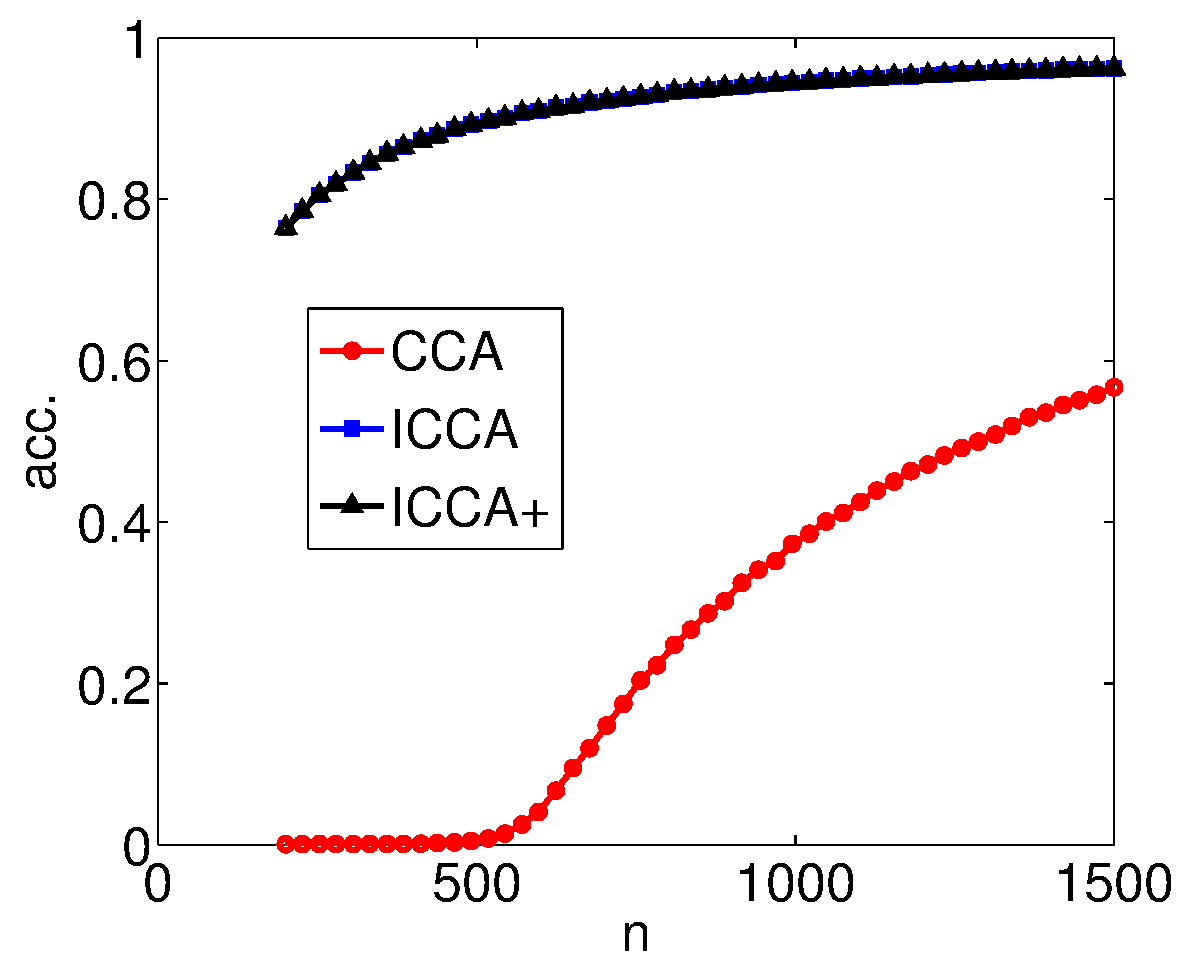
\includegraphics[width=0.4\textwidth]{chpt5_icca_vect/figs/asilomar_n.pdf}  
  \caption{Accuracy plots as a function of $n$ for a rank-2 setting where $\kx=\ky=2$,
      $p=200$, $q=250$, $\Tx=\Ty=\diag(16,4)$, $\Pxy=\diag(0.9,0.5)$, $V_K=I_2$, and
      non-identity $U_K$ defined in (\ref{eq:chpt5:uk}). Accuracy is defined in
      (\ref{eq:chpt5:cca_vect_acc}). We plot the accuracy of the first canonical vector
      for CCA, ICCA, and \iccaps.}
  \label{fig:chpt5:n_sweep}
\end{figure}

Figure \ref{fig:chpt5:theta_sweep} explores the effect of the value of $\Tx$ on the
accuracy of the canonical vectors. As $n\approx p+q$, the canonical vectors of empirical
CCA are essentially random and do not improve with an increase in SNR, which is very
undesirable. However, ICCA and \iccap are able to avoid this performance loss and the
accuracy of their canonical vectors increase with $\theta$, as desired. Again, the
performance of ICCA and \iccap are essentially identical. 

\begin{figure}
  \centering
  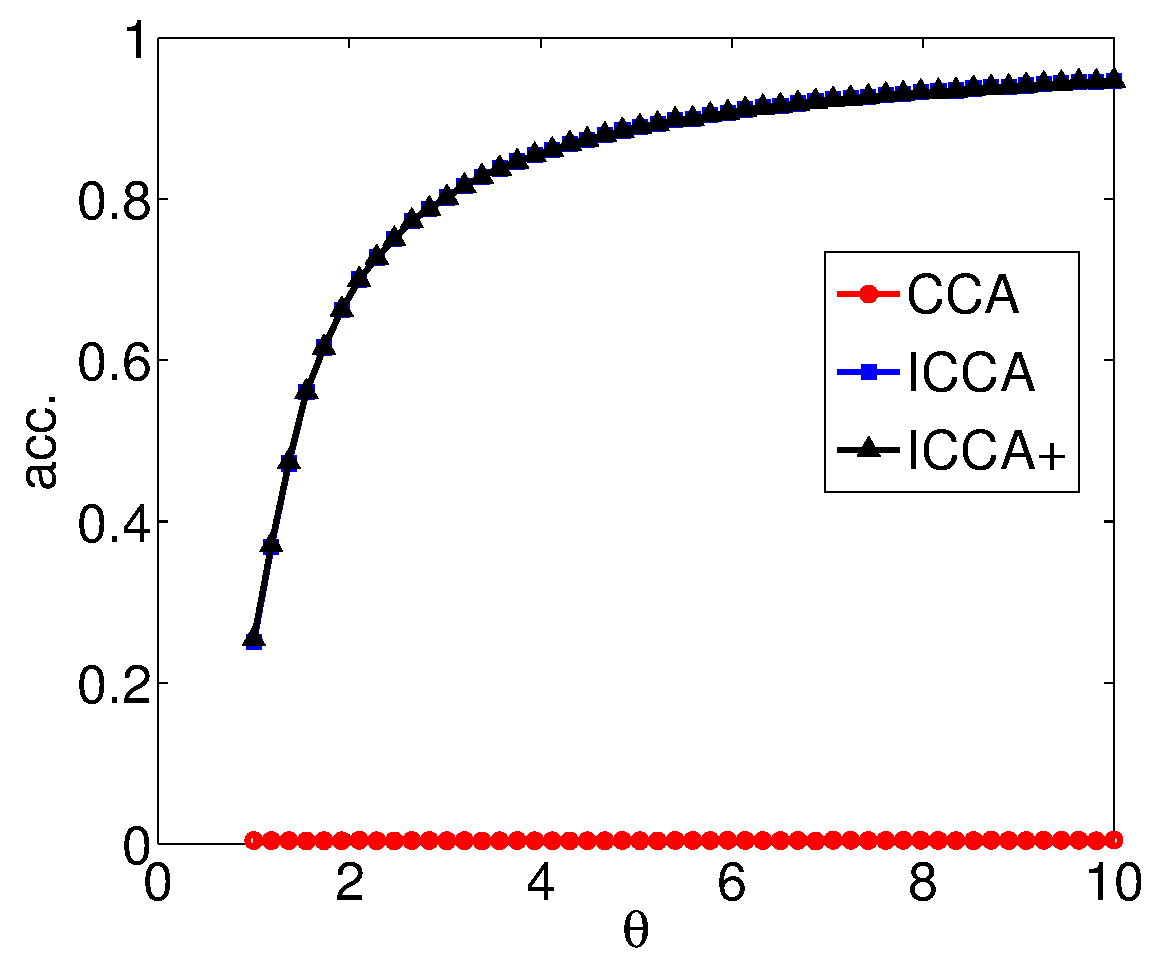
\includegraphics[width=0.4\textwidth]{chpt5_icca_vect/figs/asilomar_theta.pdf}  
  \caption{This is the same setting as Figure \ref{fig:chpt5:n_sweep} except we
    keep a fixed $n=500$ and sweep $\theta$ such that
    $\Tx=\Ty=\diag(\theta,0.8\times\theta)$. }
  \label{fig:chpt5:theta_sweep}
\end{figure}

Figure \ref{fig:chpt5:k_sweep} explores the effect of the value of $\kxhat$ on the
accuracy of the canonical vectors. Again, empirical CCA returns essentially random
canonical vectors. The canonical vectors of both ICCA and \iccap improve upon empirical
CCA, however, \iccap is more robust to overestimation of $\kxhat$. In this setup $\kx=2$
and we see that \iccap is able to place less weight on these inaccurate signal subspaces
that are included because $\kxhat$ overestimates $\kx$.

\begin{figure}
  \centering
  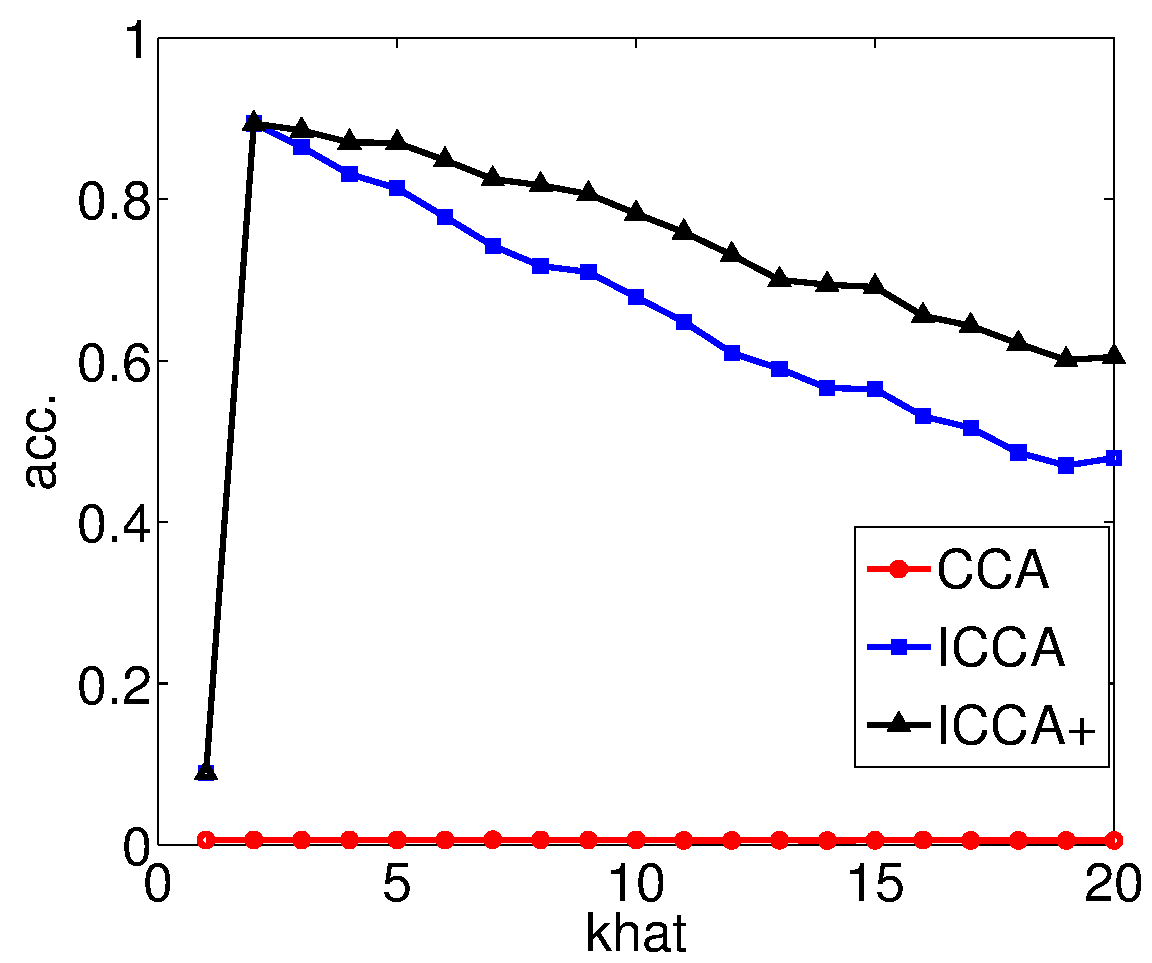
\includegraphics[width=0.4\textwidth]{chpt5_icca_vect/figs/khat_sweep.pdf}  
  \caption{This is the same setup as Figure \ref{fig:chpt5:n_sweep} except we keep a fixed
    $n=500$ and sweep of $\kxhat$.}
  \label{fig:chpt5:k_sweep}
\end{figure}

\section{Conclusion}\label{sec:chpt5:conc}

In this paper we considered the problem of estimating canonical vectors in Canonical
Correlation Analysis. We saw that in the low-sample, high dimensionality regime, the
canonical vectors returned by empirical CCA are very inaccurate. We saw that Informative
Canonical Correlation Analysis can overcome much of this performance loss by trimming data
matrices to include only \textit{informative} components. The canonical vectors of both
empirical CCA and ICCA take a linear combination of the signal subspace. By optimizing
this linear combination, our new algorithm, \iccap, can systematically improve the
accuracy of the canonical vectors and is more robust to overestimation of the rank of the
signal subspace. In future work we will consider the theoretical performance of \iccap,
extend the algorithm to missing data, and provide rigorous proofs of all results.
